\chapter{Conclusions}\label{C:conclusions}

This chapter aims to be a corollary of the whole project. And, this is done focusing on each one of the topics previously treated, which are related to prototype a cloud real-time media production platform:

\section{LiveMediaStreamer}

As seen in previous chapter \ref{H:platformDeploymentAndDemonstrations}, LiveMediaStreamer is performing properly and seems to be able to fit as the core part for real-time video and audio streams manipulation.

Figures \ref{F:isoCPU} and \ref{F:gsavgcpu} trace what is the scalability of the core in terms of stream processing capabilities. This means that if for an audio and video stream treatment (figure \ref{F:idsc}) the average CPU usage is around the 4\% and for four couples of audio and video streams treatment (figure \ref{F:gdsc}) the CPU usage is around the 23\% of an eight core CPU, then LMS becomes suitable to be treated as a reliable and a scalable core framework. And this is also remarked due to the fact of not suffering of data losses inside the pipeline (figures \ref{F:isoaplb} and \ref{F:gsalb}). But, it's important to note that in the video mixing pipeline there are accumulated losses, which, as said, appear due to its transitory time. Although, figure \ref{F:gsvpalbd} showcases a constant value which means that this data losses are not incrementing in time, so the system is stable.

\begin{figure}[!htb]
\begin{center}
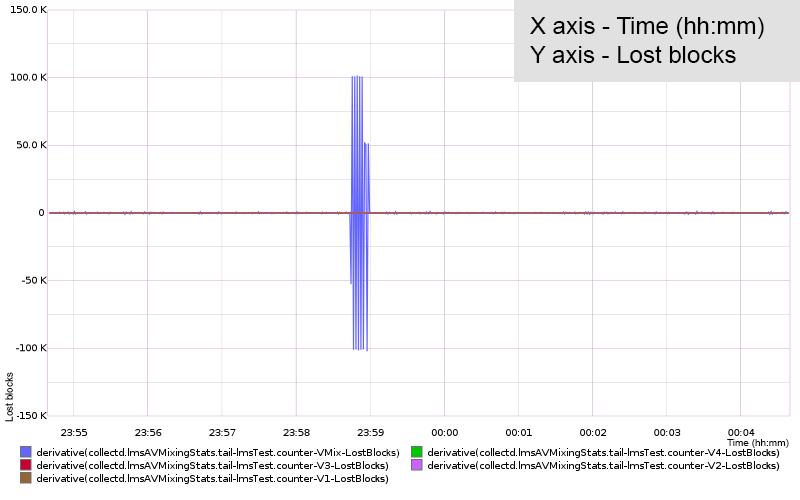
\includegraphics[width=0.70\textwidth]{./images/testAVMix/AVMixVideoLostBlocsDerivative.png}
\caption{Generic scenario - video path accumulated lost blocs derivative}
\label{F:gsvpalbd}
\end{center}
\end{figure}

Moreover, a topic related to development continuity of the LMS framework it's demonstrated that the selected third party libraries are suitable to continue being used (i.e.: Live555, LibAV/ffmpeg, x264 and OpenCV, among others). And, also regarding debugging the LMS, thanks to the metrics gathering system implemented it is possible to know which filters are critical or which should be improved.

It's also important to remark that thanks to the developments done related to metrics gathering and the tools deployed around the LMS have helped detecting issues that might not be detected in near future but could be problematic. For example, figure \ref{SF:S5} showcased that the processing time for the audio "receiver to mixer" path was not working properly due to not cleaning up the queues when the source is sending in a pseudo-live mode (i.e.: a loop, a periodic reinitialization of the audio stream).

Finally, to point out that the generic scenario, which is doing audio and video mixing of multiple inputs, showcases that the video pipeline introduces around 80 milliseconds of processing time. However, most of this introduced delay is due to the encoder (i.e.: x264 library) and the mixer (i.e.: OpenCV library) filters (the "mixer to trasmitter" path).

\section{Collectd and Graphite}

This tools selection for the monitoring layer is a good choice when the goal is to have a lightweight and highly configurable system. And this is thanks to the community behind both projects.

A critical issue about clustering such tools (i.e.: Collectd clustering) is how its bandwidth usage may affect the whole system performance. Figures \ref{F:tscbu} and \ref{F:avmscbu}, which are a filtered whireshark capture of the UDP stream bandwidth usage from the Collectd client to the Collectd+Graphite server, showcases that despite the huge amount of parameters to be sent the communication protocol is lightweight and is not an issue that the system might suffer from. In the worst case (i.e.: generic scenario) the bandwidth usage average is below 70 kbps.

\begin{figure}[!htb]
\begin{center}
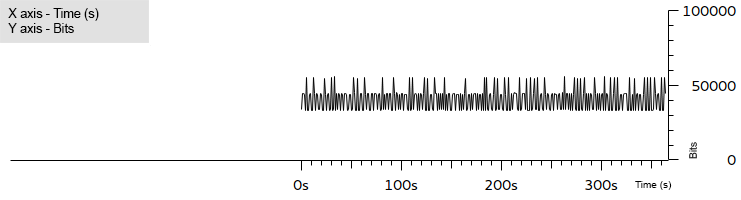
\includegraphics[width=0.70\textwidth]{./images/testStats/testStatsDocker/collectdBWbits.png}
\caption{Transcoder scenario - Collectd bandwidth usage (bits per second)}
\label{F:tscbu}
\end{center}
\end{figure}

\begin{figure}[!htb]
\begin{center}
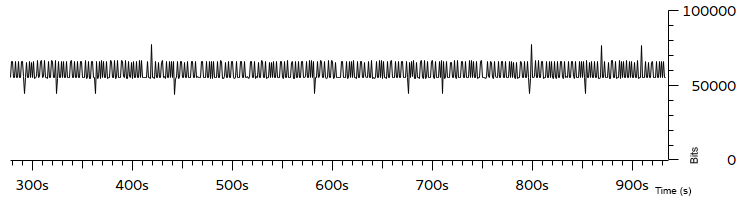
\includegraphics[width=0.70\textwidth]{./images/testAVMix/collectdBWbits.png}
\caption{Audio and video mixer scenario - Collectd bandwidth usage (bits per second)}
\label{F:avmscbu}
\end{center}
\end{figure}

Regarding the Graphite tools it's important to remark its huge amount of utilities to present and treat the metrics, which help to carry out proper graphical data minding. Moreover, to point out that it has compatibility with external tools in order to implement alarm systems or near real-time actuators over the system which is monitoring to. This fact is a key point in order to implement a cloud real-time media production platform service. 

Regarding the amount of data to be stored, thanks to the RRD (i.e.: database) system, once the periodicity and granularity of time points are defined the required storage capacity is known and remains constant in time. This is a key point due to the fact of not affecting the system performance because of the HDD usage.

There is a last point to take into account about Graphite, which is its capability to offer its graphics and specific data through its HTTP API. This means that specific applications are able to display in many ways its performance in near real-time.

\section{Docker}

Regarding this virtualization system implemented, it has demonstrated to be a proper tool to encapsulate each one of the required pieces of the platform in order to develop, test, distribute and play with them.

Moreover, Docker ease this platform to become a multiplatform tool, which means that any piece of this prototype can be executed in any OS which Docker gives support (i.e.: currently supported OS are Linux/Unix, MacOSX and Windows).

To point out that thanks to this tool, this platform becomes fast to scale due to its fast startup, restart and shutdown times. And this is also due to its ease to quickly replicate any containerized application or service, if required. 

Despite its strengths, it's not still a mature technology (the company behind, called dotCloud, and Docker project itself were born in 2013) but it's evolving really fast. And, this is demonstrated by the high growth that its community is taking place year by year. 

An example to be considered, which should be solved by Docker itself or through external solutions, is about security issues. This is mainly due to the fact that when running a containerized LMS this container does not completely isolate LMS from the security considerations of running it directly on the host, in fact it adds more security considerations. The most important of these is that the Docker daemon's API does not require any kind of authentication. It is important to make sure to have good firewall configured to isolate the host machine from outside the host, or it might be controllable from externals. 

Also, to take into account that Docker's bridged networking as well as mounted filesystem support allows for possible security holes into and out of the container itself, but it also might happen with traditional virtualization. Of course, the topic of container security is an extensive subject, but it's an issue to be strongly considered when creating a container in order to keep the security of Docker (and LXC) for granted.

\section{Platform}

Although previous tools might work properly and fit in a cloud environment the problem isn't at all solved. 

What has been developed and tested is what can be called the tip of the iceberg of a cloud real-time media production platform. Therefore, the outcomes of this project are specific tools/solutions which are suitable to be used together or separated, which lead to implement new specific and higher level tools. 


\section{Next steps}

Once this project finishes new user requirements will be gathered and new developments will be proposed. However, the main premise will remain to continue evolving as a set of tools as much configurable as possible.

Also, in order to improve some filter steps it is already proposed to work over GPGPUs. In this case, OpenCV is already offering specific APIs to work over CUDA which are of interest. Moreover, such implementations will lead to develop UHD video pipelines.

Regarding the network side and thanks to the implemented APIs it seems feasible to analyse possibilities to deploy these project tools within SDN environments which should improve management and resource optimization.

Next steps are also related to implement new codec and new media formats in order to be up to date. 

In order to improve streaming robustness, a FEC implementation is also a key point for next steps enhancements of the overall platform. There are specific and proprietary solutions but it is proposed to implement the already standard described in RFC 5109 (RTP Payload Format for Generic Forward Error Correction)

Moreover, in order to offer a complete set of tools for private media production use cases and to maintain specific license agreements (i.e.: IPR - Intellectual Property Rights) it is also proposed to implement DRM (Digital Rights Management) technology.

Finally, to point out that in order to follow the premise to be as open as possible it's proposed to create a web site of the LMS framework in order to start building a community of users and developers.